\chapter{Periodograms}
\label{ch:axions-periodograms}
The space of possible axion--induced signals is spanned by their amplitude (the strength of the coupling) and their frequency (the axion mass). The problem is therefore naturally set in the frequency domain. We perform the analysis in two steps. First, we transform the measurements from the time domain into the frequency one by evaluating a \emph{periodogram} of it. The second step, the statistical treatment, is then easy.

In this section, we present the statistical methods we use. We start by defining the \emph{periodogram}, which serves as a transition from time to the frequency space, natural for looking for oscillations. Next we proceed to discuss the statistical properties of the periodogram, which lays the basis for this analysis.

For the sake of pedagogy we will discuss the methodology on a simple example.



\section{Definition}
A \emph{periodogram} is an estimator of the power spectrum. It has been proposed as the preferred way to treat periodic signals as early as 1898~\cite{Schuster1898}. In its simplest form it is the squared magnitude of the discrete Fourier transform. Lomb and Scargle have independently described a method one can construct a statistically well--behaving periodogram for non-uniformly sampled data with unequal error--bars: the Least Squares Spectral Analysis (LSSA)~\cite{Scargle1982}. It is also known as the Lomb--Scargle periodogram.

Many packages readily offer procedures to evaluate Lomb--Scargle periodograms~\cite{scipy,astropy}. They could not, however, be used directly as the analysis deviated in details from the standard procedure. We had to take a low--level approach, instead.

\begin{figure}
  \centering 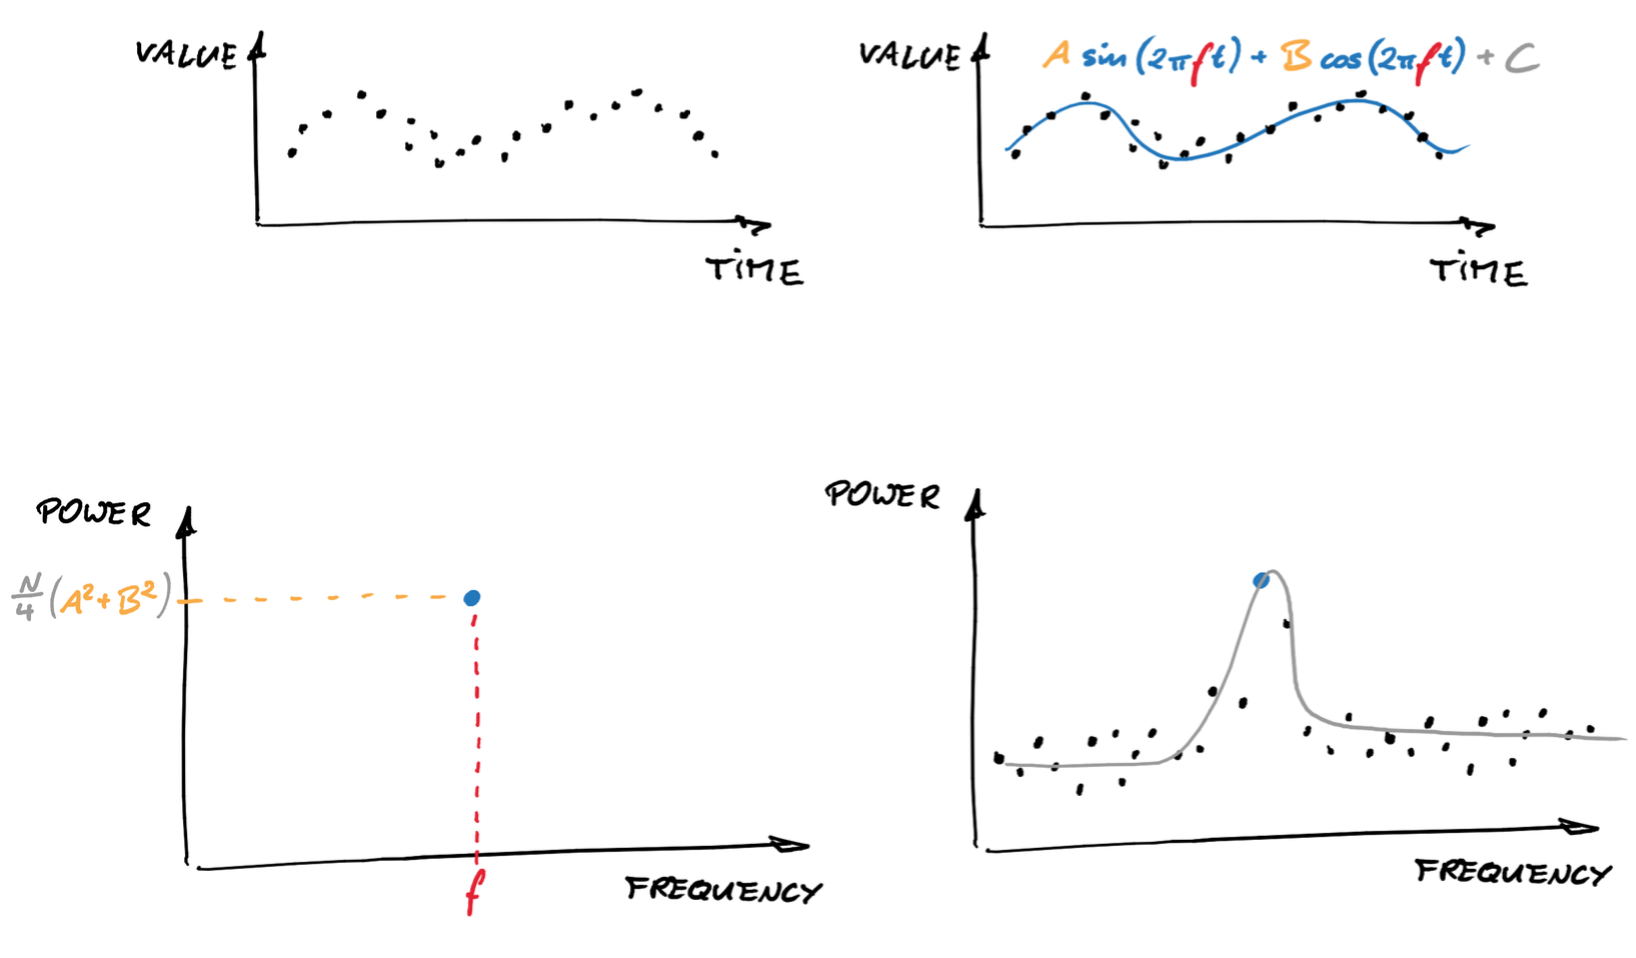
\includegraphics[width=\linewidth]{gfx/axions/LSSA}
  \caption{The LSSA periodogram, a function of frequency, is constructed by performing a linear least--squares fit at each of those frequencies.}
  \label{fig:LSSA_overview}
\end{figure}

To evaluate the LSSA periodogram at a circular frequency $\omega$, one performs a linear least--squares fit (hence the name) to the data with a function
\begin{equation}
  A\,\mathrm{cos}(\omega t) + B\,\mathrm{sin}(\omega t) + C \ ,
\end{equation}
where $A$, $B$ and $C$ are free parameters. The estimator of power $P(\omega)$ is then defined as
\begin{equation}
  P(\omega) := \frac{N}{4} \, \left( A^2 + B^2 \right) \ ,
\end{equation}
where $N$ is the number of data points. Different scaling factors may be used. We use the one of \cite{Scargle1982}, where the height of $\sqrt{P(\omega)}$ at the noise--bed corresponds numerically to the size of the error--bars squared, if they are all equal. LSSA, in contrast to the fast fourier transform (FFT), does not require windowing, because it is explicitly phase--aware. A graphical overview of the method is shown in Fig.\,\ref{fig:LSSA_overview}. Throughout the analysis, the figure of merit is either the power $P(\omega)$ or, interchangeably, its square root \emph{amplitude}. The latter has conveniently the same unit an the time series.

We will now follow an analysis of a simple example, shown in Fig.\,\ref{fig:basic_signal}. Despite being simple, is has already some properties of the actual dataset. The measurements are not equally spaced. They are grouped in 10--second long bunches, 20 seconds apart. Inside a bunch a measurement is taken every 2~seconds with a \unit[0.3]{s} jitter. The length of each measurement is 1~second with a \unit[0.1]{s} jitter. The error--bars are all size 1 in the arbitrary unit. An oscillating signal with an amplitude 0.7 and frequency \unit[0.17]{Hz}. Each measurement averages the signal over its duration.

\begin{figure}
  \centering 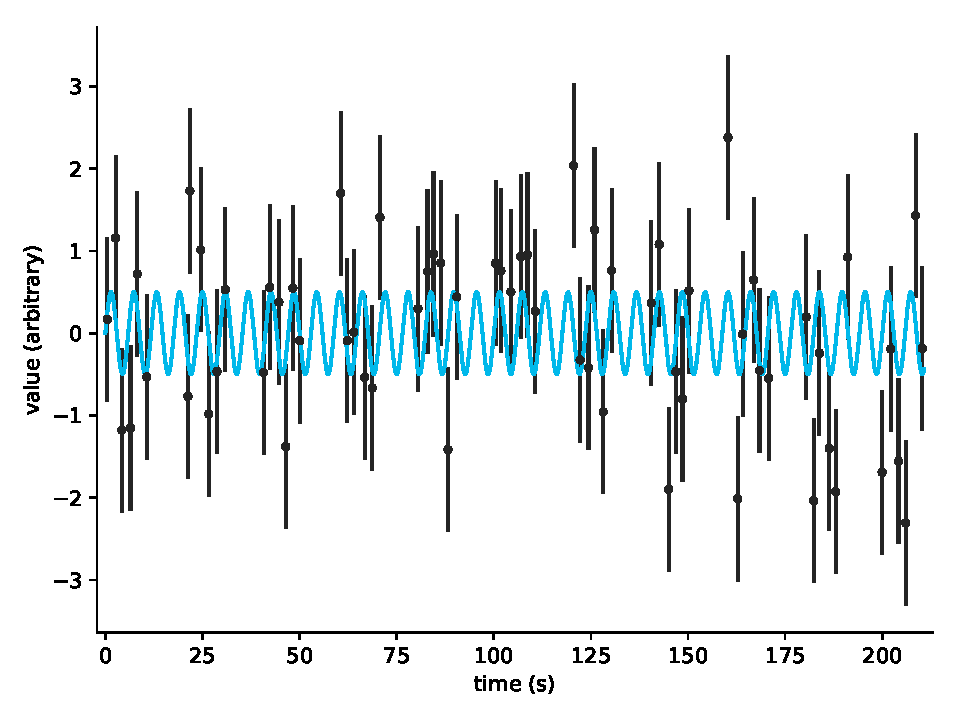
\includegraphics[width=0.8\linewidth]{gfx/axions/basic_signal.pdf}
  \caption{A simple signal generated just for the purpose for explaining the general scheme of periodogram analysis.}
  \label{fig:basic_signal}
\end{figure}

We proceed to evaluate the LSSA periodogram of this time series. The immediate question is: for which frequencies to evaluate the power? In case of equally--spaced series the upper limit is the \emph{Nyquist frequency}, equal to the half of the sampling rate~\cite{Shannon1949}. It is not the case when the sampling is not uniform. In practice we can expect little sensitivity to oscillations faster than the period over which each signal is averaged, \unit[1]{s} in the example. On the low side the limit is zero, which corresponds to the constant offset (an LSSA fit of a horizontal line, which is equivalent to calculating the average of the points).

When choosing the spacing between the frequencies we consider the the \emph{spectral resolution}, defined as the inverse span of the dataset. It roughly defines the minimal frequency difference between two signals that is distinguishable. In Fig.\,\ref{fig:basic_periodogram} there are two periodograms: evaluated at frequencies a spectral resolution apart (black dots), and one evaluated a thousand times more densely (the orange line). As no structure on a scale finer the the spectral resolution can be accessed, the orange line simply "connects" the black dots smoothly.

\begin{figure}
  \centering 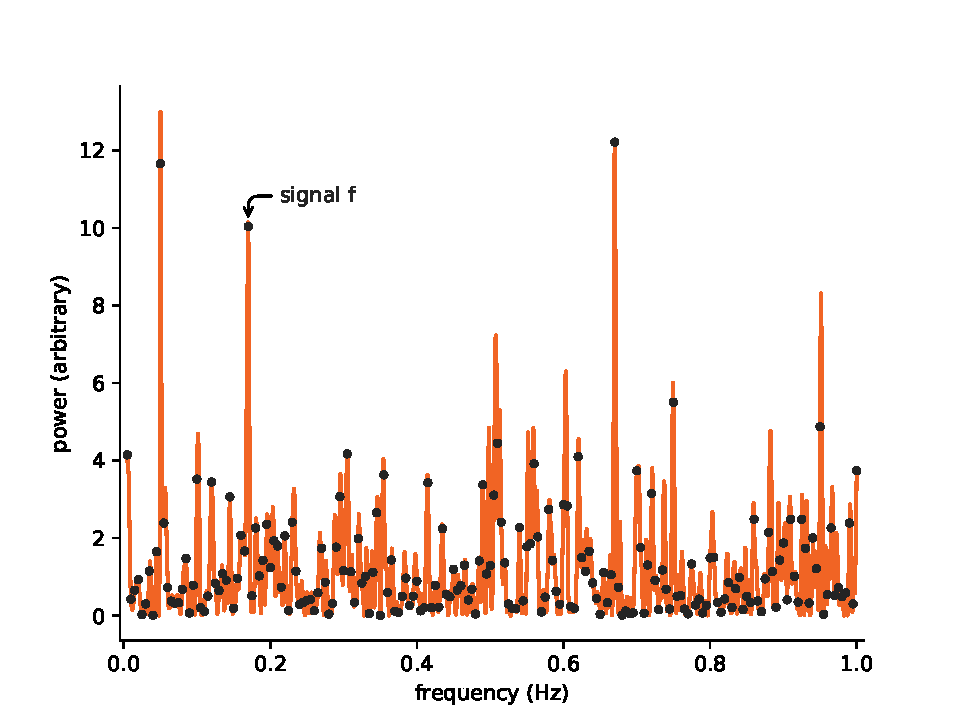
\includegraphics[width=0.8\linewidth]{gfx/axions/basic_periodogram.pdf}
  \caption{Two periodograms of the time series in Fig.\,\ref{fig:basic_signal}. One evaluated at frequencies a spectral resolution apart (black dots), and one evaluated a thousand times more densely (the orange line). As no structure on a scale finer the the spectral resolution can be accessed, the orange line simply "connects" the black dots.}
  \label{fig:basic_periodogram}
\end{figure}

In particular it is interesting to consider the difference between the 0 (offset) and the next frequency. Oscillations with a period longer than the span of the time series  appear in the series as a linear drift, if the measurements were taken in the linear part of the sine, or a quadratic change, if taken in the apex. Fitting such an oscillation is then equivalent to looking for a up--to--second--order drift in the data. Naturally, we expect the sensitivity to quickly worsen for these very long oscillations.

Fig.\,\ref{fig:basic_periodogram_loglog} shows the same two periodograms in a log--log scale. This scale is often used, as the potential signals span orders of magnitude in both frequency and amplitude. Unfortunately, it can lead to misunderstandings. Specifically, the noise appears to increase in amplitude with frequency. It is a purely cognitive effect. The spacing of the points is linear, so on a logarithmic scale the density of points increases for high amplitudes, making the extreme deviations more likely to appear in the same plot area, despite the noise amplitude being the same.

\begin{figure}
  \centering 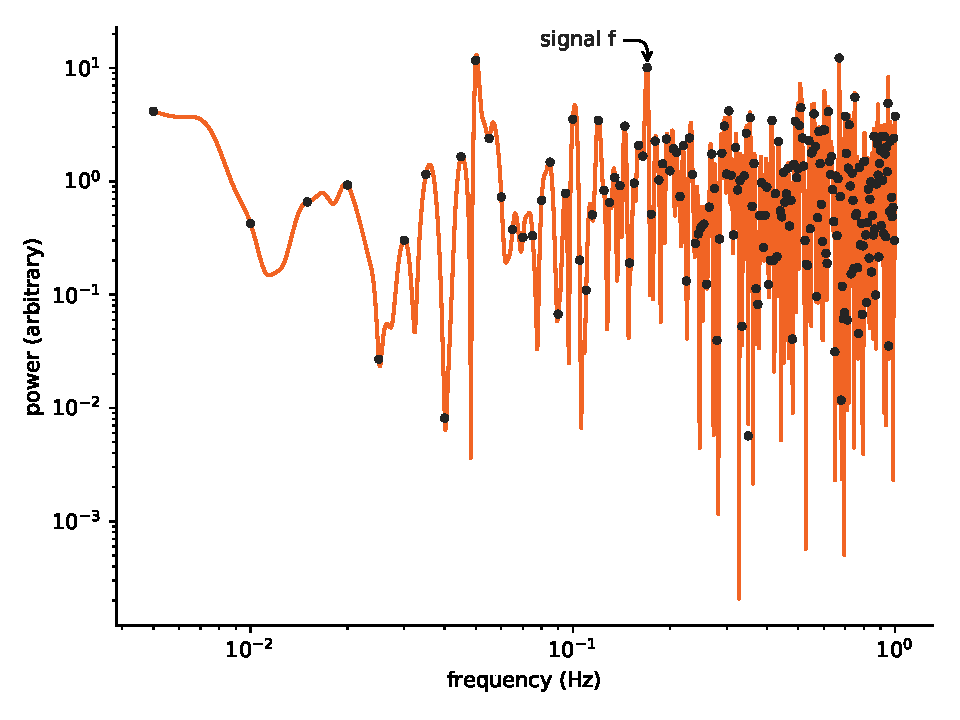
\includegraphics[width=0.8\linewidth]{gfx/axions/basic_periodogram_loglog.pdf}
  \caption{Two periodograms of the time series in Fig.\,\ref{fig:basic_signal}. One evaluated at frequencies a spectral resolution apart (black dots), and one evaluated a thousand times more densely (the orange line). As no structure on a scale finer the the spectral resolution can be accessed, the orange line simply "connects" the black dots. The periodogram is plotted on a log--log scale. The amplitude of the noise appears to be increasing with frequency, but it is not true. Only the density of the evaluated points increases, making the extreme deviations more pronounce.}
  \label{fig:basic_periodogram_loglog}
\end{figure}

An oscillation in the time series produces a peak in the periodogram. The position of the peak is the frequency of the oscillation, the width corresponds to the coherence of the signal. However, we see in the periodogram many peaks besides the one corresponding to the oscillation used when generating the data. Some are even bigger and there are many smaller ones. In the next section we will consider what, besides an oscillating signal, may give rise to a peak. Most importantly a way of determining whether a peak is caused by an oscillation is presented.




\section{A null hypothesis test}
Once the periodogram of a time series is calculated we would like to know whether it contains a signal signature. A signature of a periodic signal is a peak in the periodogram. The really interesting statement is the answer to the question:

\begin{center}
  \emph{How likely is it that the highest peak in the periodogram is not only a random fluctuation?}
\end{center}

We are, in fact, interested in the \emph{least likely} peak, which may not be the same as the highest one. For clarity we are going to be first considering the highest peak, and explain the difference later.

To describe the question mathematically, let us denote the time series of the real data by $D$. The peridogoram is then a set of $P^D(\omega_i)$. We are interested in \emph{the maximum of the periodogram}:
\begin{align}
  P_{max}^D &:= \mathrm{max}_i\,P^D(\omega_i) \\
  \omega_{max}^D &:= \mathrm{arg\,max}_{\omega_i}\,P^D(\omega_i)
\end{align}
The height of the maximum, $P_{max}^D$, is a statistic itself. We refer to it as \emph{global}, in contrast with the \emph{local} statistics $P^D(\omega_i)$. We consider the distribution of $P_{max}^{H_0}$ given the null hypothesis $H_0$, where the time array is an array of normally distributed random variables, with widths equal to the corresponding error--bars. The probability that a peak at least as high as the one observed arises as a random fluctuation is:
\begin{equation}
  % \mathrm{Pr}\left( P_{max}^{H_0} > P_{max}^D\ |\, H_0 \right) \ .
  \mathrm{Pr}\left( P_{max}^{H_0} > P_{max}^D \right) \ .
\end{equation}
This value is called the \emph{false alarm probability} (see eg. \cite{Pandola2004}). It can be numerically calculated with the Monte Carlo method by generating random data according to the null hypothesis (Fig.\,\ref{fig:generating_null_hypothesis_periodogram}) and counting the relative number of cases when $P_{max}^{H_0} > P_{max}^D$. To claim a discovery, the \emph{false alarm probability} has to be at most in the range of $2.87\,\cdot\,10^{-7}$ (so--called 5--sigma) \cite{PDG2014}.

\begin{figure}
  \centering 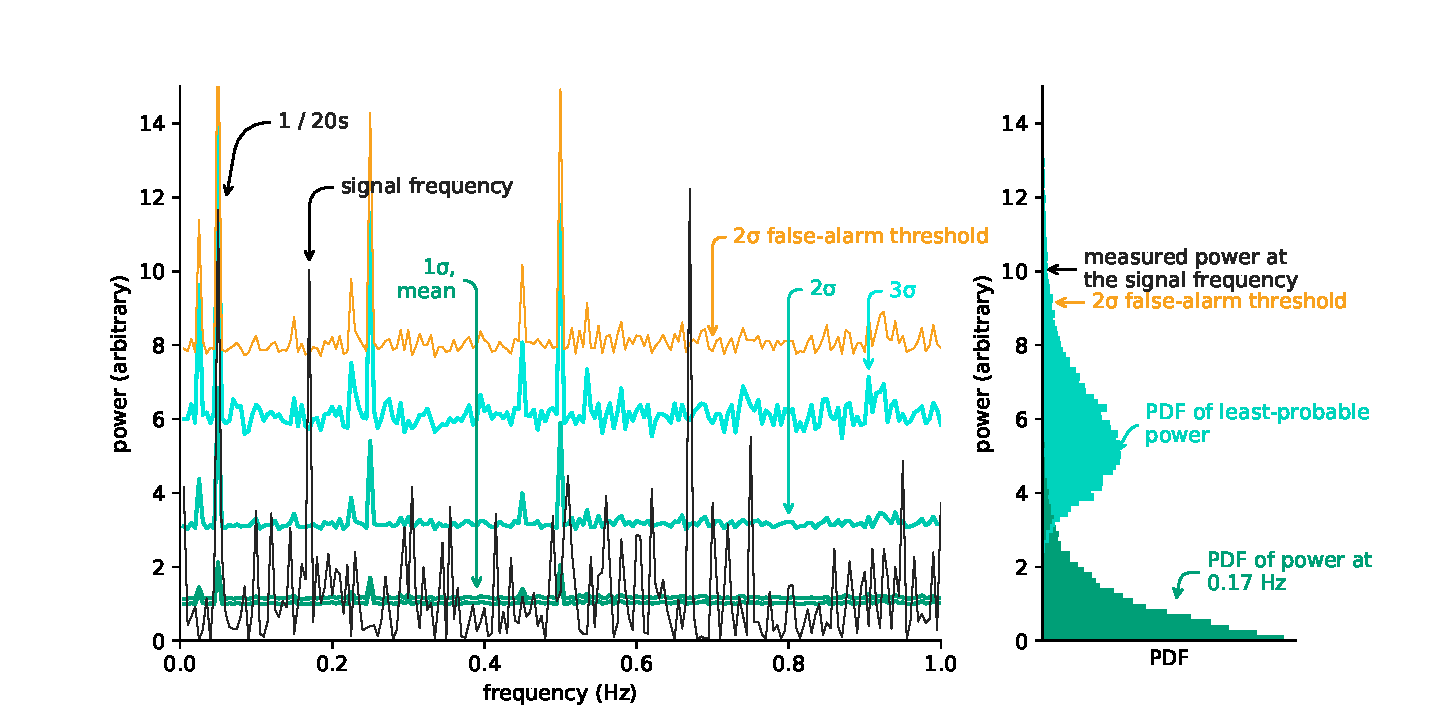
\includegraphics[width=\linewidth]{gfx/axions/basic_detection.pdf}
  \caption{A simple signal generated just for the purpose for explaining the general scheme of the analysis.}
  \label{fig:basic_detection}
\end{figure}

% \begin{figure}
%   \centering
%   \subfloat
%   % [The not--yet--real data tested against hypothetical signals. Each pixel is one signal hypothesis. The white line connects points of 95\% C.L., surrounding an exclusion region. Note how deep into low amplitudes the line goes for couple of frequencies. See the text for the explanation.]
%   {%\label{fig:axions_exclusion}
%   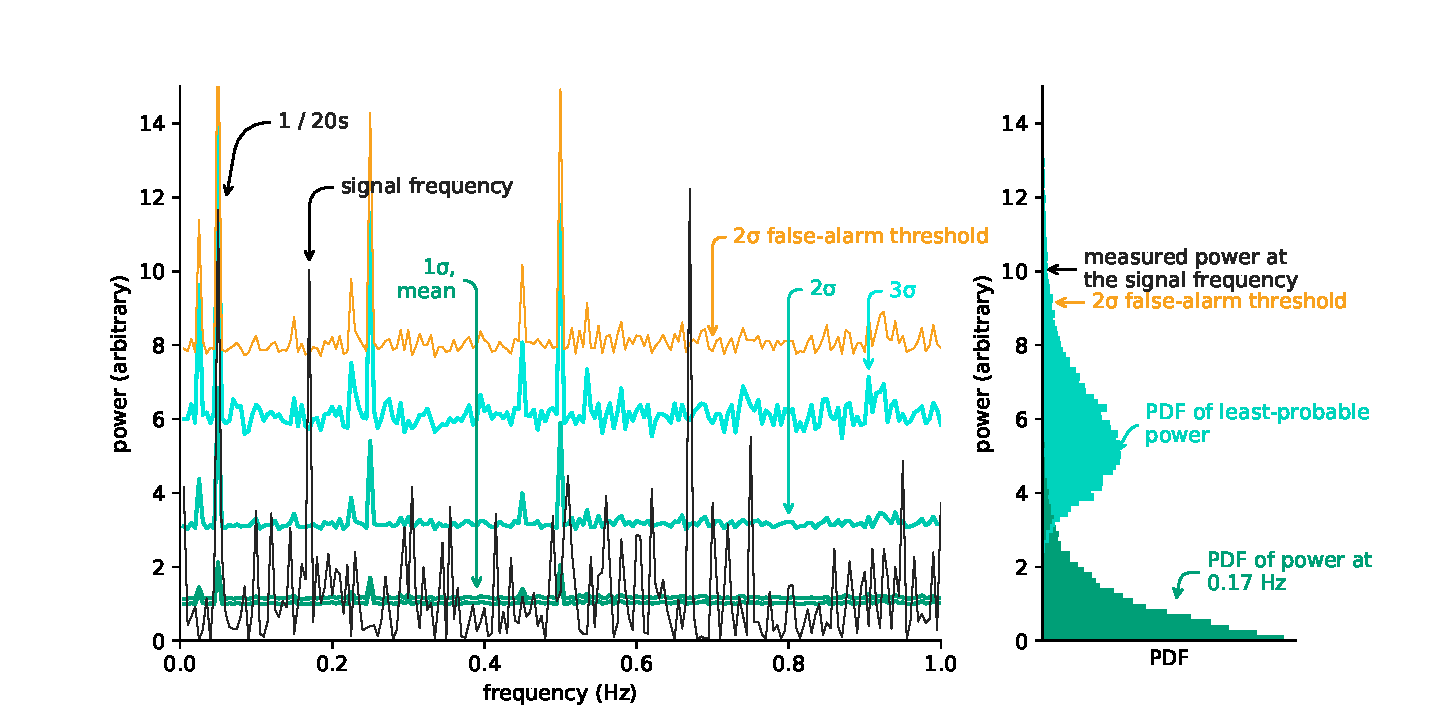
\includegraphics[width=.45\linewidth]{gfx/axions/basic_detection.pdf}}
%   \quad
%   \subfloat
%   % [The not--yet--real data tested against hypothetical signals using the \emph{CLs method}, in which hypotheses to which the experiment is not sensitive to get a statistical penalty. ]
%   {%\label{fig:basic_detection}
%   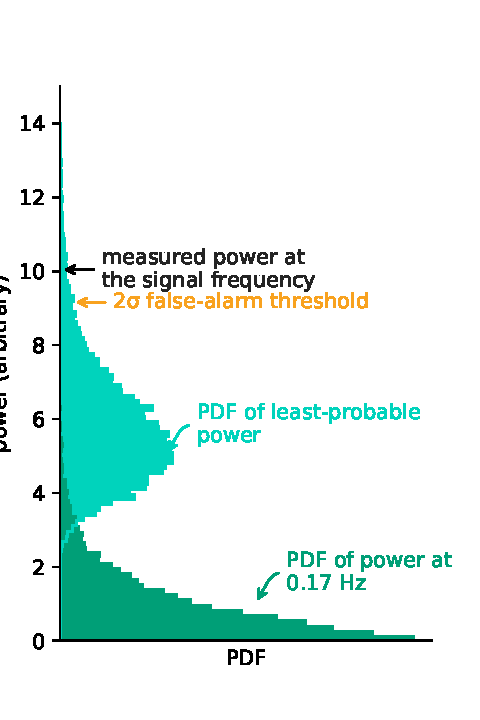
\includegraphics[width=.45\linewidth]{gfx/axions/basic_detection_histogram.pdf}}
%   \caption{Exclusion region --- signals that can be excluded at 95\% confidence level.}
%   \label{fig:basic_detection}
% \end{figure}

It should be stressed that the distribution of $P_{max}$ is very different from the one of $P(\omega_{max})$. By looking for the highest peak, we check a big number of random variables $P(\omega_i)$ and pick a very special one --- the one that does lie the furthest in the tail of the distribution. The distribution of $P_{max}$ thus is centred around much higher values, as shown in Fig.\,\ref{fig:max_power_distribution}.

The question is what is the \emph{global} p-value of the least likely peak in the data--set being compatible with $H_0$. If the points of the periodogram were not correlated, this would be a simple case of many hypothesis testing \cite{Algeri2016}. The local p-values $p_i$ are, by definition, uniformly distributed. The CDF of a maximum of a set of uncorrelated variables is a product of their CDFs \note{MR: Cite Papoulis 1965, 7.1, application 3 - taken from Scargle III a)}. So in this case we have:
\begin{align}
  F_p(p) &= p \\
  F_{p_{max}}(p) &= p^N \\
  &\text{with}\ p' := 1 - p :\\
  F_{p_{min}}(p) &= 1 - F_{p'_{max}}(p') = 1 - (1 - p)^N \label{eq:Fpmin}\\
\end{align}
where $N$ is the number of frequencies. Correlations in the periodogram effectively lower $N$. If three dice are rolled in a way that two always give the same result, this is the same as rolling two dice when minimum roll is concerned. To quantify that, we exploit the fact that we can do fast Monte Carlo and \emph{simulate} the whole process: generating many signals assuming the null--hypothesis and calculating the p-value of the least--likely peak. Thereby we can estimate the CDF of $p_{\mathrm{min}} \, | H_0$, which we call $F^g$. Then the \emph{global} p-value is given by:
\begin{equation}
  p^g = F^g(p_{\mathrm{min}}^D)
\end{equation}

We can further determine \emph{false--alarm} thresholds. Traditionally, they are chosen to be at p-values of the normal distribution at $n \,\sigma$. The \emph{global} threshold p-value we call $p^g_{f.a.}$. The \emph{local} threshold p-value is:
\begin{equation}
  p_{f.a.} = \left( F^g \right)^{-1}(p^g_{f.a.})
\end{equation}
For each frequency the threshold power can be calculated:
\begin{equation}
  P^{f.a}_i = F_{P_i}^{-1}(1 - p_{f.a.})
\end{equation}
We claim a statistically significant discovery if the periodogram of the $d_n$ time--series crosses the 5--sigma false--alarm threshold.

The amount of Monte Carlo samples can be reduced, if the CDFs can be extrapolated. Effects like unequal error--bars and measurements of non--negligible duration causes them to deviate from the strictly derived equations in \cite{Scargle1982}. Nevertheless, we assume that functional form of the tails is preserved. Under the null hypothesis $F_{P_i}$ has form $1 - e^{-P}$ \cite{Scargle1982}. For $F^g$ we assume a form of Eq.\,(\ref{eq:Fpmin}), where $N$ is a parameter that we have to fit to account for correlations in the periodogram.

In Fig.\,\ref{fig:ILL_detection} we present the periodogram of a fake ILL dataset (geneated with the same run timings and uncertainties as in the real dataset, with run EDM values generated according to gaussian distribution with mean of $0$ and standard deviation equal to that run's uncertainty). We decided not to analyse the real data set until we are fully happy with the method.

\begin{figure}[h!]
  \begin{center}
    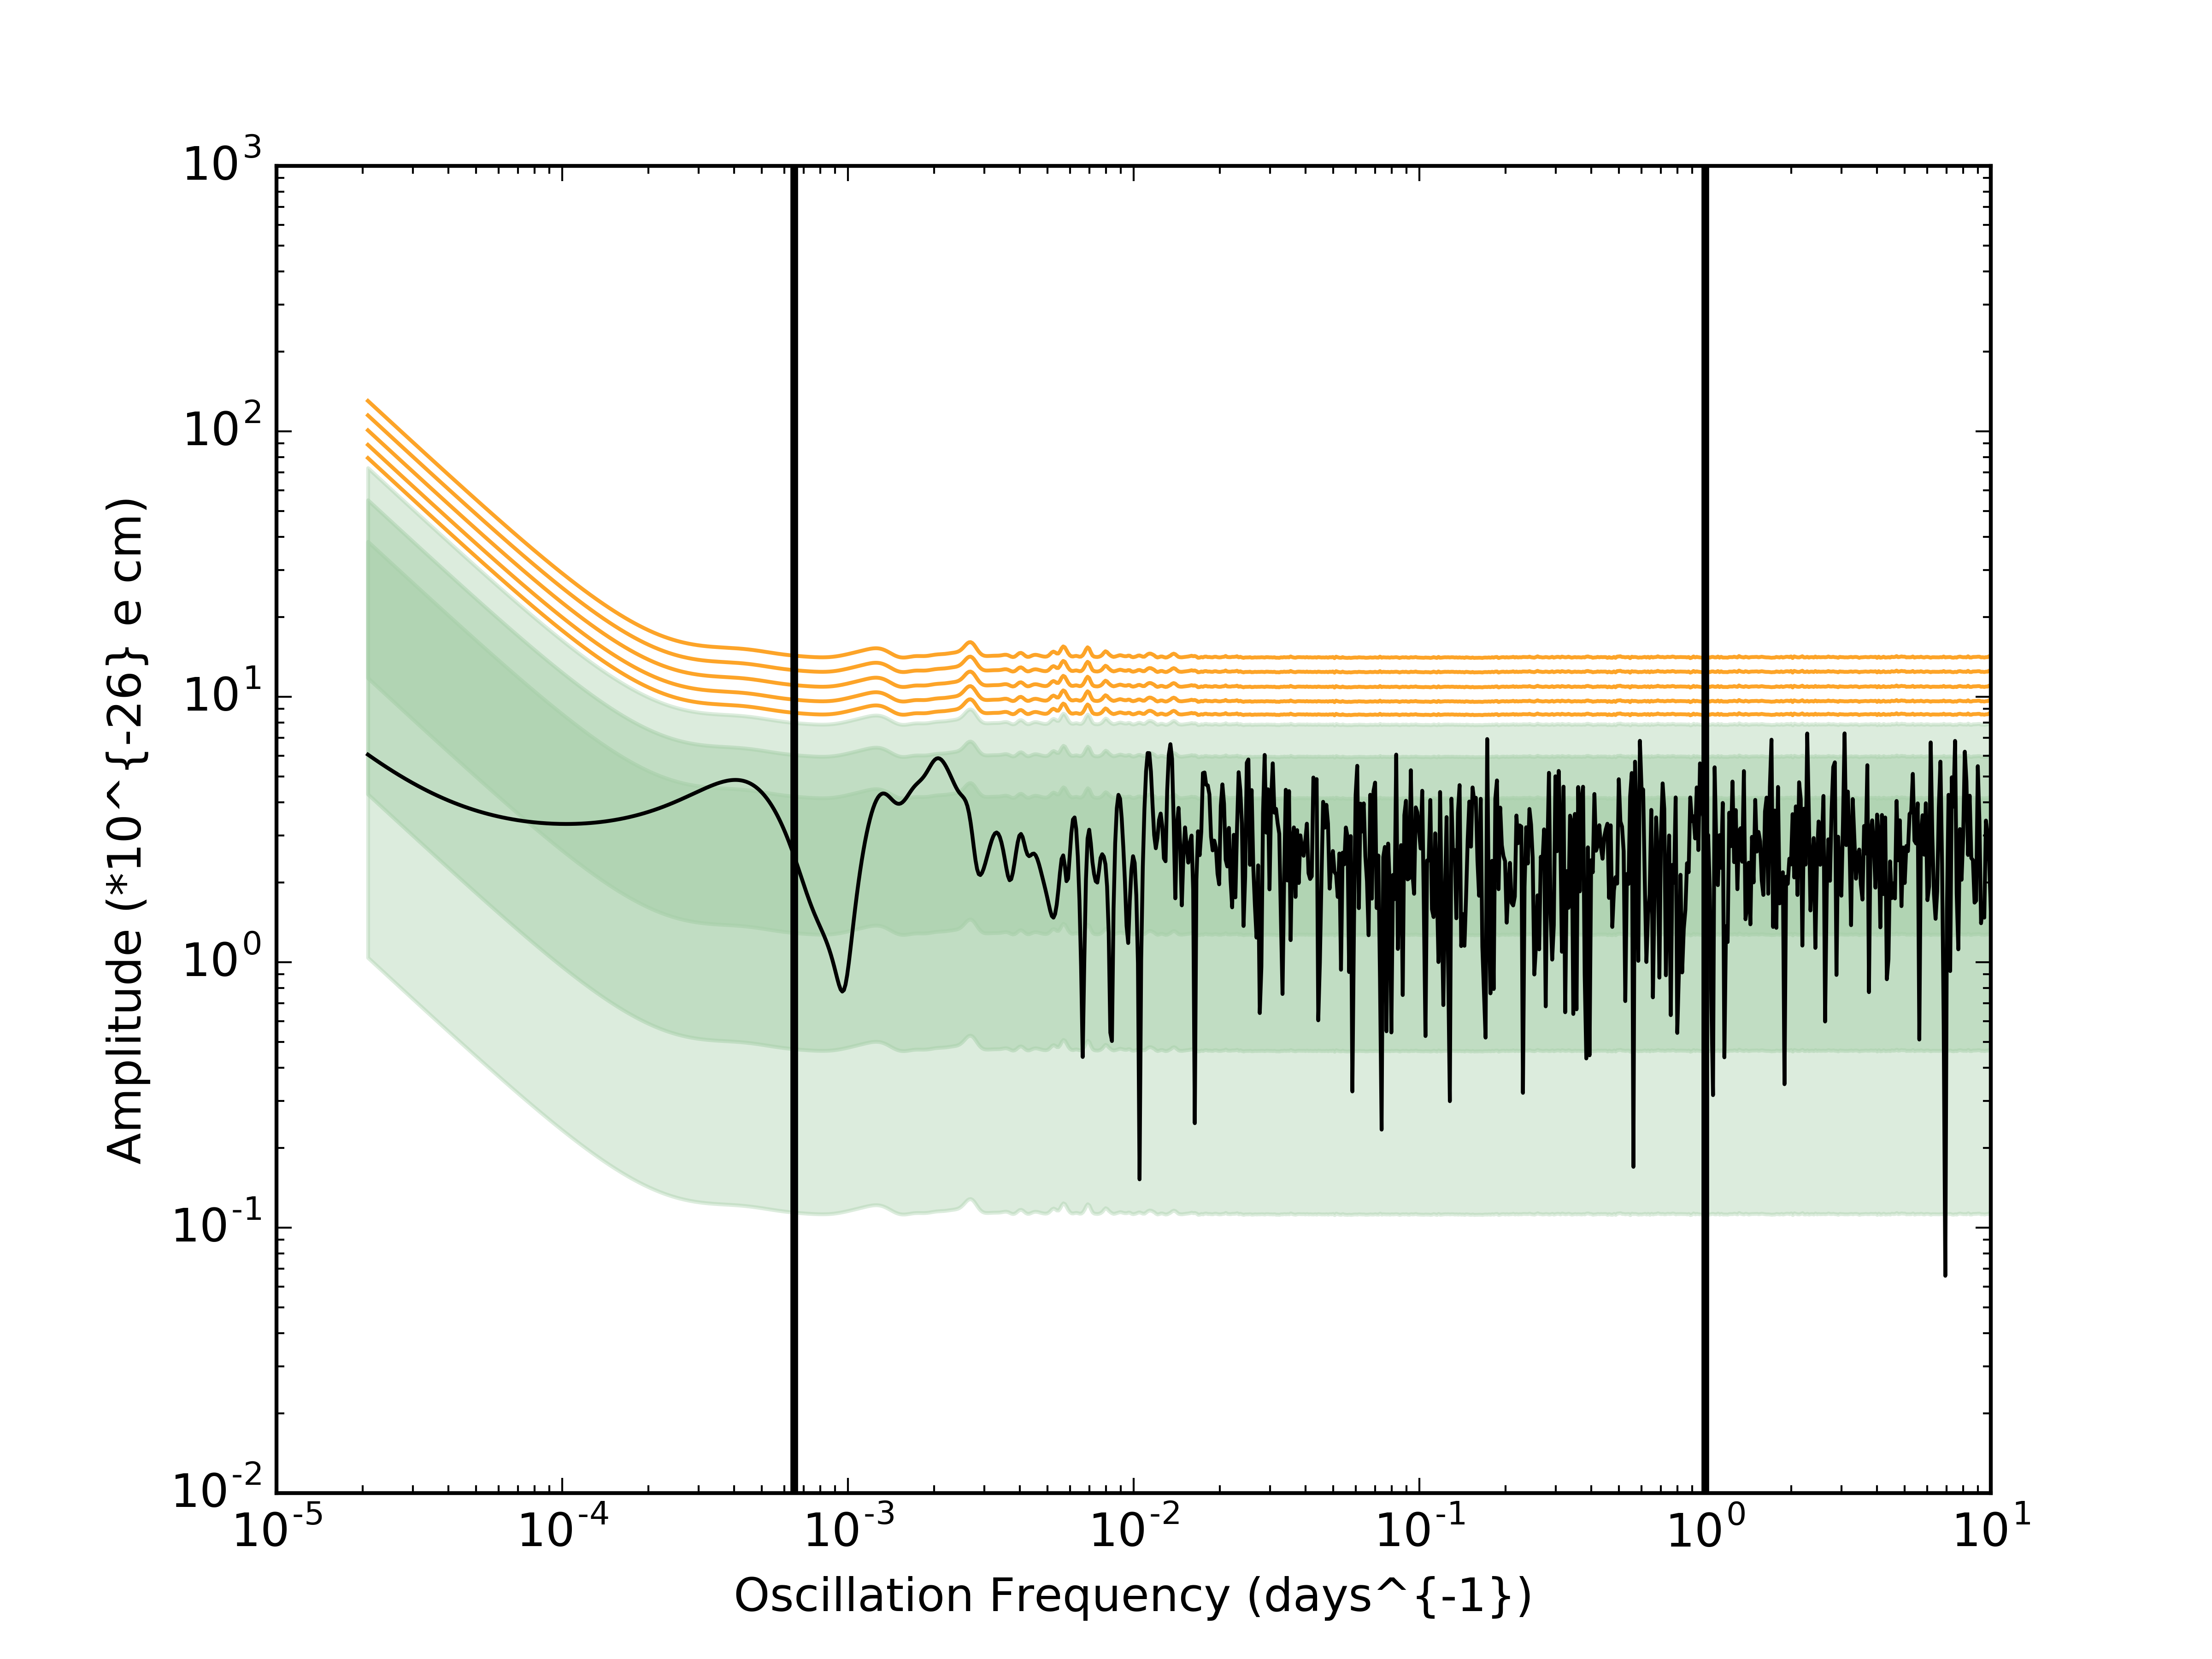
\includegraphics[width=\columnwidth]{gfx/axions/ILL_detection_Periodogram.png}
    \caption{Periodogram of a fake ILL dataset. The green bands represent the distribution of the periodogram given the null hypothesis. The orange lines are 1-, 2-, 3-, 4-, 5--sigma false--alarm thresholds.}
    \label{fig:ILL_detection}
  \end{center}
\end{figure}





\section{Signal hypotheses tests}
Should no claim for a discovery be possible, the next question to ask is:
\begin{center}
  \emph{Which oscillations would produce a visible peak, but did not, and can be thus excluded?}
\end{center}
In order to answer this question, the data need to be tested against being compatible with a number of model signal hypotheses. As an oscillation is characterised by its amplitude and frequency, the space of the hypotheses to test is two--dimensional.

The probability that a hypothetical oscillation of amplitude $A$ and frequency $\omega$ would produce more power at $\omega$ then observed is:
\begin{equation}
  \mathrm{Pr}\left( P(\omega) > P^D(\omega)\ |\, H(\omega, A) \right) \ .
\end{equation}
This probability is the \emph{confidence level} (C.L.) at which the hypothesis $H(\omega, A)$ can be rejected. Figure\,\ref{fig:axions_signal_rejection} presents comparing a not--yet--real data power spectrum with a hypothetical signal. This test may be performed many times, each covering a \emph{pixel} of the space of possible hypotheses, forming an image as in Fig.\,\ref{fig:axions_exclusion}. The set of hypotheses excluded at a certain C.L. (often 95\%) forms an \emph{exclusion region}.

% \begin{figure}
%   \myfloatalign
%   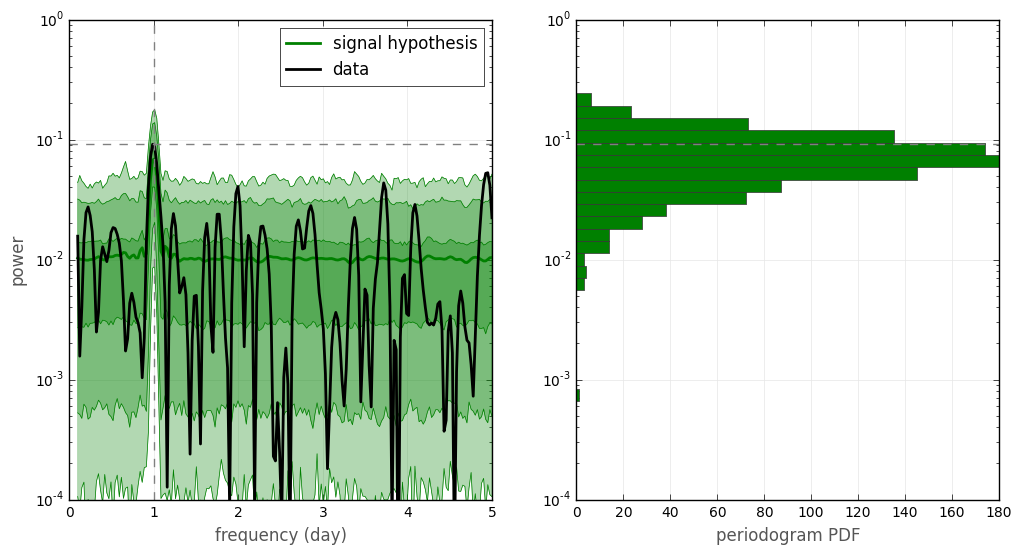
\includegraphics[width=.8\linewidth]{gfx/axions/axionMC_signal_hypothesis_rejection}
%   \caption
%   [...]
%   {
% \textsc{Left:} A periodogram of not--yet--real data on top of distribution of a periodogram of a hypothetical signal (green). \textsc{Right:} The distribution of power of the hypothetical signal at its model frequency.}
%   \label{fig:axions_signal_rejection}
% \end{figure}

\begin{figure}
  %FIXME directly copied from Elise's presentation on the 2015 PSI collaboration meeting
  \myfloatalign
  \subfloat
  [The not--yet--real data tested against hypothetical signals. Each pixel is one signal hypothesis. The white line connects points of 95\% C.L., surrounding an exclusion region. Note how deep into low amplitudes the line goes for couple of frequencies. See the text for the explanation.]
  {\label{fig:axions_exclusion_noCls}
  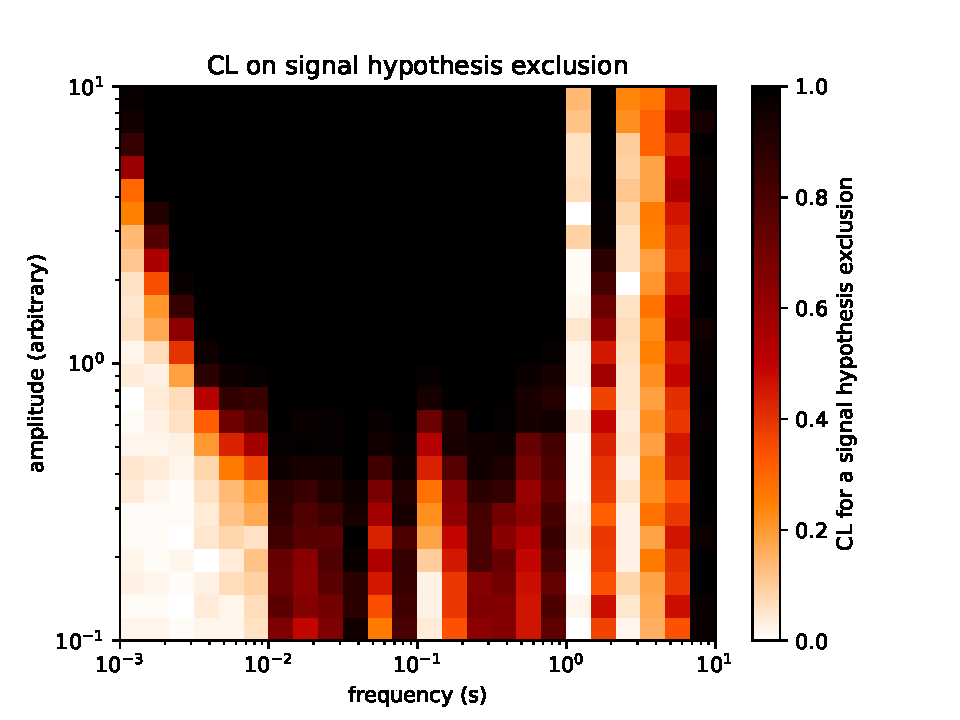
\includegraphics[width=.45\linewidth]{gfx/axions/basic_exclusion_noCls.pdf}}
  \quad
  \subfloat
  [The not--yet--real data tested against hypothetical signals using the \emph{CLs method}, in which hypotheses to which the experiment is not sensitive to get a statistical penalty. ]
  {\label{fig:axions_exclusion}
  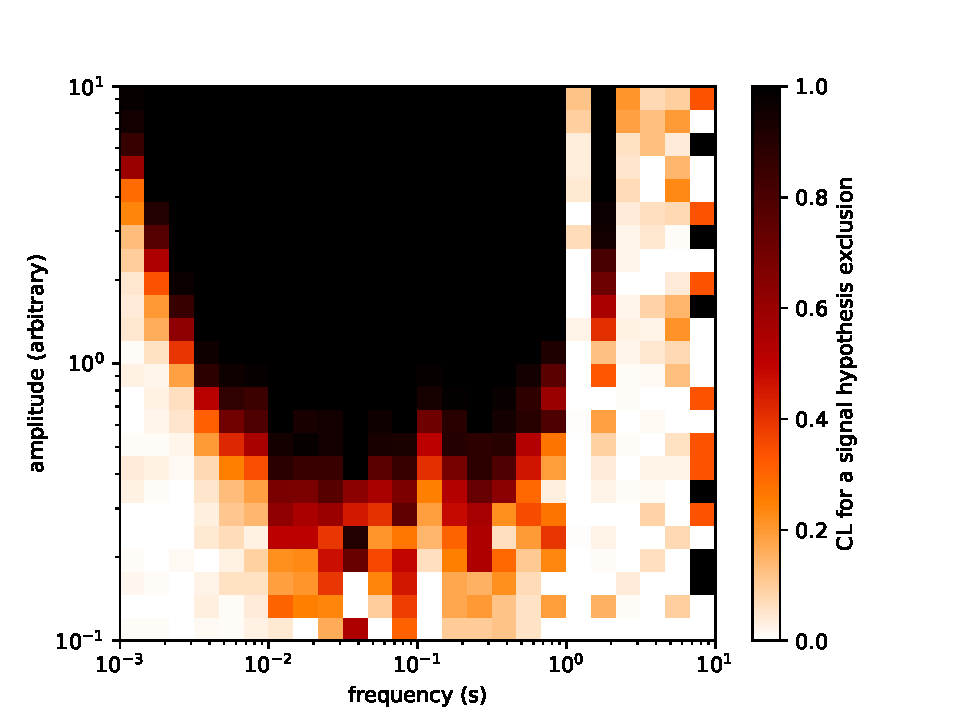
\includegraphics[width=.45\linewidth]{gfx/axions/basic_exclusion.pdf}}
  \caption{Exclusion region --- signals that can be excluded at 95\% confidence level..}
  \label{fig:axions_exclusions}
\end{figure}

The exclusion region, depicted by a white line in Fig.\,\ref{fig:axions_exclusion}, is exhibits a number of thin peaks going down in very low amplitudes. Seemingly for some frequencies signals with amplitude far below the sensitivity of the experiment are excluded. This is disturbing. Consider, however, that as the power was evaluated for many frequencies, inevitably at some of them, roughly 5\%, the power is low enough to be rejected at 95\%~C.L. even when tested against a white noise. However completely fine from the statistical point of view, physicists do not accept a situation, where a hypothesis is rejected based on an experiment which was not sensitive to it. One possible solution is called the \emph{CLs method}. The method is defined, as well the problem itself discussed, in the booklet of Particle Data Group~\citep{Group2014}. With use of the \emph{CLs method} the exclusion final region is obtained, as shown in Fig.\,\ref{fig:axions_exclusion_CLs}.
